\documentclass{beamer}
\usepackage[utf8]{inputenc}

\usetheme{Madrid}
\usecolortheme{default}
\usepackage{amsmath,amssymb,amsfonts,amsthm}
\usepackage{txfonts}
\usepackage{tkz-euclide}
\usepackage{listings}
\usepackage{adjustbox}
\usepackage{array}
\usepackage{tabularx}
\usepackage{gvv}
\usepackage{lmodern}
\usepackage{circuitikz}
\usepackage{tikz}
\usepackage{graphicx}

\setbeamertemplate{page number in head/foot}[totalframenumber]

\usepackage{tcolorbox}
\tcbuselibrary{minted,breakable,xparse,skins}

\definecolor{bg}{gray}{0.95}
\DeclareTCBListing{mintedbox}{O{}m!O{}}{%
breakable=true,
listing engine=minted,
listing only,
minted language=#2,
minted style=default,
minted options={%
linenos,
gobble=0,
breaklines=true,
breakafter=,,
fontsize=\small,
numbersep=8pt,
#1},
boxsep=0pt,
left skip=0pt,
right skip=0pt,
left=25pt,
right=0pt,
top=3pt,
bottom=3pt,
arc=5pt,
leftrule=0pt,
rightrule=0pt,
bottomrule=2pt,
toprule=2pt,
colback=bg,
colframe=orange!70,
enhanced,
overlay={%
\begin{tcbclipinterior}
\fill[orange!20!white] (frame.south west) rectangle ([xshift=20pt]frame.north west);
\end{tcbclipinterior}},
#3,
}
\lstset{
language=C,
basicstyle=\ttfamily\small,
keywordstyle=\color{blue},
stringstyle=\color{orange},
commentstyle=\color{green!60!black},
numbers=left,
numberstyle=\tiny\color{gray},
breaklines=true,
showstringspaces=false,
}

\title
{9.5.6}
\date{October 7, 2025}
\author
{EE25BTECH11043 - Nishid Khandagre}

\begin{document}

\frame{\titlepage}

\begin{frame}{Question}
Find the sum and product of the roots of the quadratic equation
$2x^2-9x + 4 = 0$.
\end{frame}

\begin{frame}{Theoretical Solution}
Given quadratic equation:
\begin{align}
    y=2x^2 - 9x + 4
\end{align}
Representing this equation as a conic section
\begin{align}
    \vec{x}^{\top}\vec{V}\vec{x} + 2\vec{u}^{\top}\vec{x} + f=0 \ , \  \vec{V}=\myvec{2 & 0\\0&0} \ , \  \vec{u}=\myvec{-9/2 \\ -1/2} \ ,\ f=4
\end{align}
We need to find intersection points with $y=0$, that is, the X-axis.
\begin{align}
    \vec{x}=\vec{h} + k \vec{m} \ , \ \vec{h}=\myvec{0 \\ 0} \ , \ \vec{m}=\myvec{1 \\ 0}
\end{align}
Substituting $\vec{x} = k \vec{m}$
\end{frame}

\begin{frame}{Theoretical Solution}
\begin{align}
    k^2\vec{m}^{\top}\vec{V}\vec{m} + 2k\vec{u}^{\top}\vec{m} + f=0 \\
    \implies k= \dfrac{1}{2 \vec{m}^{\top}\vec{V}\vec{m}} \sbrak{ -2\vec{u}^{\top}\vec{m} \ \pm \ \sqrt{\brak{2\vec{u}^{\top}\vec{m}}^2 - 4 f \vec{m}^{\top}\vec{V}\vec{m}}}\\
    \implies k= \dfrac{1}{\vec{m}^{\top}\vec{V}\vec{m}} \sbrak{ -\vec{u}^{\top}\vec{m} \ \pm \ \sqrt{\brak{\vec{u}^{\top}\vec{m}}^2-f \vec{m}^{\top}\vec{V}\vec{m}}}
\end{align}
Now,
\begin{align}
    \vec{u}^{\top}\vec{m} = \myvec{-9/2 & -1/2}\myvec{1 \\0} = -9/2 \\
    \vec{m}^{\top}\vec{V}\vec{m}=\myvec{1 & 0}\myvec{2 & 0\\0&0}\myvec{1 \\ 0} = 2
\end{align}
\end{frame}

\begin{frame}{Theoretical Solution}
\begin{align}
    k= \dfrac{1}{2} \sbrak{ -\brak{-9/2} \ \pm \ \sqrt{ \brak{-9/2}^2 - 4 \cdot 2}}\\
    k= \dfrac{1}{2} \sbrak{ \dfrac{9}{2} \ \pm \ \dfrac{7}{2}}
\end{align}
This gives us two values for $k$:
\begin{align}
    \implies k_1= 4\\
    \implies k_2= \dfrac{1}{2}
\end{align}
Substituting $k$ into $\vec{x}$, we get the roots:
\begin{align}
    \vec{x} = \myvec{4 \\ 0} \text{ OR } \vec{x}=\myvec{1/2 \\ 0}
\end{align}
\end{frame}

\begin{frame}{Theoretical Solution}
This implies that the roots of $2x^2 -9x + 4 =0$ are $4$ and $\frac{1}{2}$.
Now, calculate the sum and product of these roots:

Sum of the roots:
\begin{align}
\text{Sum} = 4 + \frac{1}{2} = \frac{9}{2}
\end{align}
Product of the roots:
\begin{align}
\text{Product} = 4 \times \frac{1}{2} = 2
\end{align}
\end{frame}

\begin{frame}[fragile]
\frametitle{C Code}
\begin{lstlisting}{c}
#include <stdio.h>

// Function to find the sum and product of the roots of a quadratic equation
// For a quadratic equation ax^2 + bx + c = 0
// Sum of roots = -b/a
// Product of roots = c/a
void calculateRootsInfo(double a, double b, double c, double *sum_of_roots, double *product_of_roots) {
    *sum_of_roots = -b / a;
    *product_of_roots = c / a;
}
\end{lstlisting}
\end{frame}

\begin{frame}[fragile]
\frametitle{Python Code (using C shared library)}
\begin{lstlisting}{python}
import ctypes
import numpy as np
import matplotlib.pyplot as plt

# Load the shared library
lib_quadratic = ctypes.CDLL("./code16.so")

# Define the argument types and return type for the C function
lib_quadratic.calculateRootsInfo.argtypes = [
    ctypes.c_double,  # a
    ctypes.c_double,  # b
    ctypes.c_double,  # c
    ctypes.POINTER(ctypes.c_double), # sum_of_roots
    ctypes.POINTER(ctypes.c_double)  # product_of_roots
]
lib_quadratic.calculateRootsInfo.restype = None
\end{lstlisting}
\end{frame}

\begin{frame}[fragile]
\frametitle{Python Code (using C shared library)}
\begin{lstlisting}
# Given quadratic equation: 2x^2 - 9x + 4 = 0
a_given = 2.0
b_given = -9.0
c_given = 4.0

# Create ctypes doubles to hold the results
sum_result = ctypes.c_double()
product_result = ctypes.c_double()
# Call the C function
lib_quadratic.calculateRootsInfo(
    a_given, b_given, c_given,
    ctypes.byref(sum_result),
    ctypes.byref(product_result)
)

sum_of_roots = sum_result.value
product_of_roots = product_result.value
\end{lstlisting}
\end{frame}

\begin{frame}[fragile]
\frametitle{Python Code (using C shared library)}
\begin{lstlisting}
print(f"For the quadratic equation {a_given}x^2 + {b_given}x + {c_given} = 0:")
print(f"The sum of the roots is: {sum_of_roots:.2f}")
print(f"The product of the roots is: {product_of_roots:.2f}")

# --- Part 2: Plotting the parabola and its roots ---
# Calculate the discriminant
delta = b_given**2 - 4 * a_given * c_given

# Find the roots (if real)
roots = []
if delta >= 0:
    root1 = (-b_given + np.sqrt(delta)) / (2 * a_given)
    root2 = (-b_given - np.sqrt(delta)) / (2 * a_given)
    roots.append(root1)
    if root1 != root2: # Add distinct root2 if it exists
        roots.append(root2)
    roots.sort() # Sort for consistent labeling
\end{lstlisting}
\end{frame}

\begin{frame}[fragile]
\frametitle{Python Code (using C shared library)}
\begin{lstlisting}{python}
# Determine plotting range based on roots or a default
if roots:
    min_root = min(roots)
    max_root = max(roots)
    # Expand the range a bit around the roots
    plot_min_x = min_root - (abs(max_root - min_root) * 0.5 + 1)
    plot_max_x = max_root + (abs(max_root - min_root) * 0.5 + 1)
    if plot_min_x == plot_max_x: # Case for a single root
        plot_min_x -= 5
        plot_max_x += 5
else: # If no real roots, use a reasonable default range
    plot_min_x = -5
    plot_max_x = 5

x_vals = np.linspace(plot_min_x, plot_max_x, 400)
y_vals = a_given * x_vals**2 + b_given * x_vals + c_given

plt.figure(figsize=(10, 6))
\end{lstlisting}
\end{frame}

\begin{frame}[fragile]
\frametitle{Python Code (using C shared library)}
\begin{lstlisting}
# Plot the parabola
plt.plot(x_vals, y_vals, label=f'${a_given}x^2 {b_given:+}x {c_given:+} = 0$', color='blue')

# Mark the roots
for i, root in enumerate(roots):
    plt.scatter(root, 0, color='red', s=100, zorder=5, label=f'Root {i+1}: {root:.2f}')
    plt.annotate(f'({root:.2f}, 0)', (root, 0), textcoords="offset points", xytext=(5,5), ha='left', color='red')

# Add x and y axes for reference
plt.axhline(0, color='black', linewidth=0.8, linestyle='--')
plt.axvline(0, color='black', linewidth=0.8, linestyle='--')
\end{lstlisting}
\end{frame}

\begin{frame}[fragile]
\frametitle{Python Code (using C shared library)}
\begin{lstlisting}
plt.xlabel('x')
plt.ylabel('y')
plt.title('Quadratic Parabola and its Real Roots')
plt.grid(True, linestyle=':', alpha=0.7)
plt.legend()
plt.ylim(min(y_vals)-abs(min(y_vals)*0.1)-1, max(y_vals)+abs(max(y_vals)*0.1)+1) # Adjust y-limits dynamically
plt.xlim(plot_min_x, plot_max_x) # Ensure x-limits are set
plt.show()
\end{lstlisting}
\end{frame}

\begin{frame}[fragile]
\frametitle{Python Code (Direct)}
\begin{lstlisting}{python}
import numpy as np
import matplotlib.pyplot as plt

def solve_quadratic_and_plot(a, b, c):
    """
    Calculates the sum and product of roots for a quadratic equation (ax^2 + bx + c = 0),
    and generates a plot of the parabola marking its real roots.
    """
    # --- Part 1: Calculate sum and product of roots ---
    # Sum of roots = -b/a
    sum_of_roots = -b / a
    # Product of roots = c/a
    product_of_roots = c / a

    print(f"For the quadratic equation {a}x^2 + {b}x + {c} = 0:")
    print(f"The sum of the roots is: {sum_of_roots:.2f}")
    print(f"The product of the roots is: {product_of_roots:.2f}")
\end{lstlisting}
\end{frame}

\begin{frame}[fragile]
\frametitle{Python Code (Direct)}
\begin{lstlisting}
    # --- Part 2: Plotting the parabola and its roots ---
    # Calculate the discriminant
    delta = b**2 - 4 * a * c

    # Find the roots (if real)
    roots = []
    if delta >= 0:
        root1 = (-b + np.sqrt(delta)) / (2 * a)
        root2 = (-b - np.sqrt(delta)) / (2 * a)
        roots.append(root1)
        if root1 != root2: # Add distinct root2 if it exists
            roots.append(root2)
        roots.sort() # Sort for consistent labeling
    else:
        print("\nNo real roots for this equation (discriminant is negative).")
\end{lstlisting}
\end{frame}

\begin{frame}[fragile]
\frametitle{Python Code (Direct)}
\begin{lstlisting}
    # Determine plotting range based on roots or a default
    if roots:
        min_root = min(roots)
        max_root = max(roots)
        # Expand the range a bit around the roots
        padding = abs(max_root - min_root) * 0.5 + 1
        if padding == 1: # Case where there's only one root or roots are identical
             padding = 2 # Ensure some sensible padding
        plot_min_x = min_root - padding
        plot_max_x = max_root + padding
    else: # If no real roots, use a reasonable default range
        plot_min_x = -5
        plot_max_x = 5

    x_vals = np.linspace(plot_min_x, plot_max_x, 400)
    y_vals = a * x_vals**2 + b * x_vals + c
\end{lstlisting}
\end{frame}

\begin{frame}[fragile]
\frametitle{Python Code (Direct)}
\begin{lstlisting}{python}
    plt.figure(figsize=(10, 6))
    # Plot the parabola
    plt.plot(x_vals, y_vals, label=f'${a}x^2 {b:+}x {c:+} = 0$', color='blue')
    # Mark the roots
    for i, root in enumerate(roots):
        plt.scatter(root, 0, color='red', s=100, zorder=5, label=f'Root {i+1}: {root:.2f}')
        plt.annotate(f'({root:.2f}, 0)', (root, 0), textcoords="offset points", xytext=(5,5), ha='left', color='red')
    # Add x and y axes for reference
    plt.axhline(0, color='black', linewidth=0.8, linestyle='--')
    plt.axvline(0, color='black', linewidth=0.8, linestyle='--')
    plt.xlabel('x')
    plt.ylabel('y')
    plt.title('Quadratic Parabola and its Real Roots')
    plt.grid(True, linestyle=':', alpha=0.7)
    plt.legend()
\end{lstlisting}
\end{frame}

\begin{frame}[fragile]
\frametitle{Python Code (Direct)}
\begin{lstlisting}{python}
    if len(y_vals) > 1 and np.std(y_vals) > 1e-6:
        y_min_plot = np.min(y_vals)
        y_max_plot = np.max(y_vals)
        y_padding = abs(y_max_plot - y_min_plot) * 0.1
        if y_padding == 0: y_padding = 1
        plt.ylim(y_min_plot - y_padding, y_max_plot + y_padding)
    else: # Fallback for cases with very flat or constant functions
        plt.ylim(min(y_vals)-2, max(y_vals)+2)
    plt.xlim(plot_min_x, plot_max_x) # Ensure x-limits are set
    plt.show()

# --- Main execution ---
# Given quadratic equation: 2x^2 - 9x + 4 = 0
a_given = 2.0
b_given = -9.0
c_given = 4.0
solve_quadratic_and_plot(a_given, b_given, c_given)
\end{lstlisting}
\end{frame}

\begin{frame}{Plot by Python using shared output from C}
\begin{figure}[H]
\centering
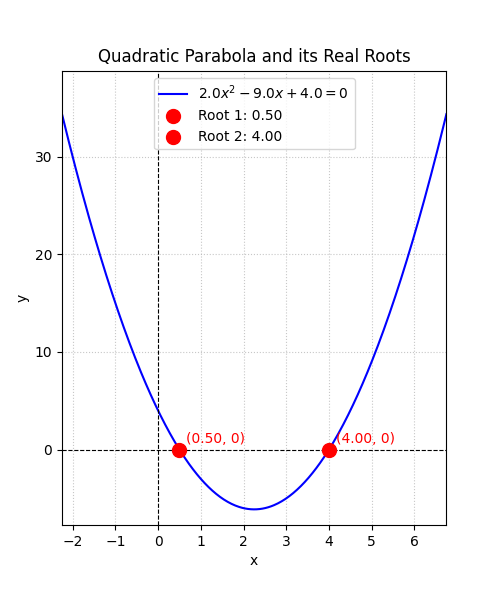
\includegraphics[width=0.6\columnwidth]{../figs/fig1.png}
\caption{}
\label{fig:1}
\end{figure}
\end{frame}

\begin{frame}{Plot by Python only}
\begin{figure}[H]
\centering
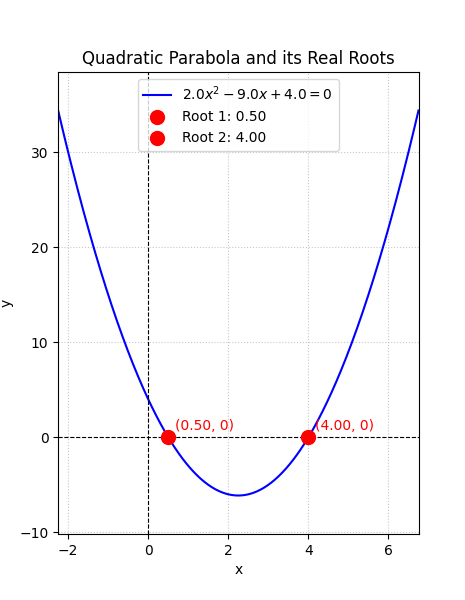
\includegraphics[width=0.5\columnwidth]{../figs/fig2.png}
\caption{}
\label{fig:2}
\end{figure}
\end{frame}

\end{document}
